
\chapter{\textsl{exploits}}
\label{chap:exploits}
	No presente capítulo, será feita uma breve análise sobre \textsl{exploits}.
	É importante salientar que, apenas conhecendo as técnicas usadas pelos atacantes
	torna-se possível criar defesas efetivas contra elas.
	Portanto, o estudo dessa matéria não constitui, de forma alguma, uma apologia
	ao ataque. Essa questão é muito bem abordada na parte I de \cite{Harris2008}, deixando
	claro que o conhecimento é uma arma importantíssima para aqueles que buscam
	uma melhoria na segurança do software.
	

	Como ponto de partida, iremos nos aprofundar um pouco mais no conceito de \textsl{exploit}.

	Para que esse tópico seja melhor ilustrado, o próximo capítulo abordará em detalhes um 
	tipo de \textsl{exploit} em específico: o \textsl{NULL pointer exploit}.

	\section{Definição}
		Conforme foi tratado na Seção \ref{sec:vuln_exploit}, o \textsl{exploit} é um conjunto de passos,
		muitas vezes materializado em um programa, capaz de tirar proveito de uma vulnerabilidade.
		Para muitos, entretanto, \textsl{exploit} é sinônimo de um código em C escrito por um \textsl{hacker}
		que tem o potencial de atacar um sistema. Essa visão, todavia, é muito limitada.
		Assim como existem diversos tipos de vulnerabilidades, há muitos meios de tirar vantagem
		delas. Por vezes, basta conhecer uma série de passos, como cliques na interface
		da aplicação alvo, para para explorar uma falha.

		
		Em \cite{Hoglund2004}, encontramos a seguinte lista de possíveis consequências
		para um \textsl{exploit} bem sucedido:
		\begin{itemize}
			\item{Exposição de dados confidenciais;}
			\item{Parada parcial ou completa do sistema(\textsl{crash});}
			\item{Execução de código injetado pelo atacante;}
			\item{Escalada de privilégios;}
		\end{itemize}
		Integridade, disponibilidade, confidencialidade.

	\section{Tipos}
		
		Listar a variedade de tipos de exploits.
		Destacar Buffer overflow, Heap overflow, Injeção de SQL, XSS.

	\section{Programação segura}
		Recomendações. Dicas do CLASP.
		Uso da ferramentas de análise estática.
	
	\section{Proteções e contra-proteções}
	\label{sec:exploit_protection}
		Existem diversas proteções para impedir um \textsl{exploit}.
		São recursos dos compiladores, das bibliotecas, do hardware e dos sistemas operacionais
		que servem de contra ponto às mais variadas técnicas que os atacantes já criaram.
		Seu principal objetivo é resguardar os sistemas mesmo que os desenvolvedores
		não tenham seguido as recomendações de segurança. De forma que, mesmo na presença de uma
		vulnerabilidade, um ataque não seja possível ou seus efeitos sejam minimizados ao máximo.
		
		
		Conforme é possível encontrar em \cite{Anley2007}, destacamos os seguintes mecanismos
		de proteção:
		\begin{enumerate}
			\item{Pilha não executável;}
			\item{W \^\ X(permissão de escrita ou de execução - nunca ambas);}
			\item{Canário para pilha;}
			\item{Reordenamento das variáveis na pilha;}
			\item{ASLR - Randomização do espaço de endereços;}
			\item{Proteções do Heap;}
			\item{Proteções do SEH;}
		\end{enumerate}

		
		A seguir, cada uma será explicada em seus aspectos fundamentais.
		\subsection{Pilha não executável}
			A primeira, pilha não executável, é uma reação natural a um dos ataques mais comuns:
			o \textsl{buffer overflow}. Há registros de propostas de pilha não executável desde 1996 -
			conforme \cite{Anley2007}(pg. 376). O \textsl{exploit} clássico sendo baseado na cópia
			de \textsl{shell code} para o buffer e posterior execução dele ficaria impraticável.
			Mas não demorou muito para os atacantes reagirem. Surgiram novas técnicas que funcionam
			mesmo quando não é possível executar o código injetado na pilha.
			Sua estratégia básica era: a partir do controle do \textsl{stack frame}, criar uma chamada
			válida para biblioteca C ou chamadas de sistema. Inicialmente, ela foi denominada \textbf{return-into-libc}.
			
			
			Essa nova técnica de \textsl{exploit} abriria caminho para uma série de outras.
		

		\subsection{W\^\ X}
			Impedir que memória com proteção de escrita seja executável e, bloquear a escrita
			para aquela que é executável é uma das melhores formas de proteção.
			Ataca justamente um princípio fundamental da maioria das técnicas de ataque: injetar código
			(escrever) e executá-lo.	
			

			Embora essa técnica seja hoje em dia conhecida pelo batismo de Theo Raadt, desenvolvedor
			e líder do projeto do OpenBSD, ela tem sua origem na década de 1970. Em \cite{Anley2007},
			é mencionado que o sistema Multics teria sido um dos pioneiros a contar com esse tipo de
			proteção. Para facilitar essa estratégia de defesa na arquitetura x86, em 2003, a AMD
			criaria o \textbf{NX(Non-eXecutable)}. Um suporte no hardware que identificasse uma página de
			memória que não pudesse ser executada. O equivalente da Intel seria o \textsl{ED(Execute Disable)}.


			Mesmo sendo uma excelente forma de impedir ataques, isolada, essa defesa não é capaz
			suficiente. Algumas técnicas derivadas de \textsl{return-into-libc} são imunes.


		\subsection{Canário para a pilha}
			Outra forma de proteção para a pilha é colocação de um canário.
			Trata-se de um valor(normalmente de 32 bits) que é posto no \textsl{stack frame}
			para identificar se houve um \textsl{overflow} na pilha.
			A figura \ref{fig:canario} ilustra essa proteção. O canário é posto para proteger
			
			\begin{figure}
				\begin{center}
					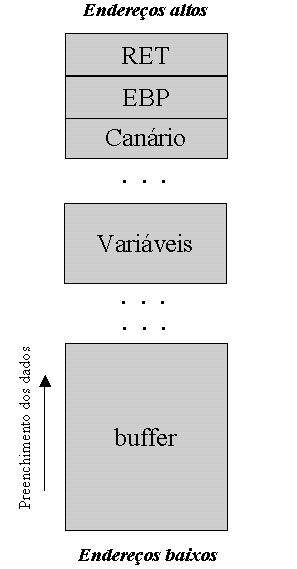
\includegraphics[width=0.30\textwidth]{canario.jpg}
					\caption{\textsl{Stack frame} protegido por canário. Fonte: \cite{Furlan2005}.}
					\label{fig:canario}
				\end{center}
			\end{figure}

		\subsection{Reordenamento de variáveis na pilha}

		\subsection{ASLR}
			O \textsl{\textbf{Address Space Layout Randomization}} implementa uma randomização
			dos endereços de forma a dificultar enormemente a vida dos atacantes.
			Bibliotecas e rotinas passam a ter endereços aleatórios e os saltos necessários
			para esses endereços ficam muito mais complexos de serem realizados.
			

			Conforme explicado anteriormente, vários \textsl{exploits} dependem de um conhecimento
			prévio dos endereços. O ASLR 

		

		
			
	
